\documentclass[11pt,a4paper]{article}

% Required Packages
\usepackage[utf8]{inputenc}
\usepackage[margin=1in]{geometry}
\usepackage{amsmath,amssymb,amsfonts}
\usepackage{graphicx}
\usepackage{booktabs}
\usepackage{hyperref}
\usepackage{xcolor}
\usepackage{listings}
\usepackage{array}
\usepackage{float}
\usepackage{tikz}
\usetikzlibrary{shapes.geometric, arrows, positioning}

% Hyperref Setup
\hypersetup{
    colorlinks=true,
    linkcolor=blue,
    filecolor=magenta,      
    urlcolor=cyan,
    pdftitle={InfraPulse: Photo-Based Defect Detection & Priority Maintenance System},
    pdfpagemode=FullScreen,
}

% Colors Setup
\definecolor{codegreen}{rgb}{0,0.6,0}
\definecolor{codegray}{rgb}{0.5,0.5,0.5}
\definecolor{codepurple}{rgb}{0.58,0,0.82}
\definecolor{backcolour}{rgb}{0.95,0.95,0.92}

% Code Listing Setup
\lstdefinestyle{mystyle}{
    backgroundcolor=\color{backcolour},   
    commentstyle=\color{codegreen},
    keywordstyle=\color{magenta},
    numberstyle=\tiny\color{codegray},
    stringstyle=\color{codepurple},
    basicstyle=\ttfamily\footnotesize,
    breakatwhitespace=false,         
    breaklines=true,                 
    captionpos=b,                    
    keepspaces=true,                 
    numbers=left,                    
    numbersep=5pt,                  
    showspaces=false,                
    showstringspaces=false,
    showtabs=false,                  
    tabsize=2
}
\lstset{style=mystyle}

\title{\textbf{InfraPulse: Photo-Based Defect Detection \& Priority Maintenance System}\\[0.5em]
\large Technical Architecture, Multi-Model Vision Consensus, and Priority Queue Formulation\\[0.3em]
\small \textbf{Takneek '26 — Mid-Prep Problem Statement} | IIT Kanpur Students' Gymkhana}
\author{\textbf{InfraPulse Engineering Team}}
\date{September 2026}

\begin{document}

\maketitle

\begin{abstract}
Buildings, hostels, hospitals, and public facilities accumulate maintenance defects such as concrete spalling, stagnant water pooling, and tile cracking that often go unreported until escalating into safety hazards or costly structural repairs. Facility teams currently rely on manual, unstructured reporting where every complaint receives identical priority regardless of actual risk. \textbf{InfraPulse} is an enterprise-grade, photo-based defect detection and automated priority maintenance web system designed to automate public infrastructure triage. Powered by a self-contained multi-model PyTorch vision ensemble (\texttt{ConvNeXt-Tiny}, \texttt{Swin-Transformer}, and \texttt{MTL Dual-Branch}), InfraPulse achieves \textbf{91.29\% test accuracy} and \textbf{0.9112 Macro F1-score} across 241 evaluation photographs. Tickets are automatically routed into isolated domain staff portals and ranked in real-time using a mathematically calibrated priority formula combining category tier base safeguards, spatial edge density severity, visible defect extent, and a strictly capped time bonus. InfraPulse operates with zero external AI service dependencies, ensuring 100\% local execution and strict adherence to Takneek '26 guidelines.
\end{abstract}

\tableofcontents
\newpage

% ---------------------------------------------------------
\section{Introduction \& Problem Statement}
% ---------------------------------------------------------

\subsection{Background}
Civil infrastructure maintenance requires timely detection and triage of physical surface defects. Manual inspection workflows suffer from significant operational bottlenecks:
\begin{enumerate}
    \item \textbf{Subjective Reporting}: Non-expert reporters provide inconsistent, qualitative descriptions of damage severity.
    \item \textbf{FIFO Queue Inefficiency}: First-In, First-Out (FIFO) queueing treats minor superficial blemishes (e.g., paint discoloration) with equal urgency to critical structural compromises (e.g., concrete spalling).
    \item \textbf{Delayed Escalation}: High-risk defects remain unnoticed in unmonitored backlogs until failure occurs.
\end{enumerate}

\subsection{Takneek '26 Requirements Mapping}
Per the Takneek '26 Problem Statement specification (\texttt{InfraPulse.pdf}), participants must deliver a fully integrated web application that accepts user defect photographs, automatically identifies defect classes, routes them into category-specific staff queues, and maintains real-time priority rankings.

\begin{table}[H]
\centering
\caption{Takneek '26 Defect Category and Queue Routing Specification}
\label{tab:ps_spec}
\begin{tabular}{llll}
\toprule
\textbf{Category} & \textbf{Target Defect} & \textbf{Tier Base} & \textbf{Domain Staff Scope} \\
\midrule
\textbf{Structural} & Spalling & 3000 pts & Concrete pillars, beams, structural masonry \\
\textbf{Functional} & Stagnant Water & 2000 pts & Drainage blockages, floor water pooling \\
\textbf{Performance} & Cracked Tiles, Paint Peeling & 1000 pts & Surface finish, aesthetic floor/wall repair \\
\bottomrule
\end{tabular}
\end{table}

\textbf{Rule Constraint}: The problem statement mandates that defect identification must be \textit{``limited strictly to what is visibly evident in the photograph, with no claims about non-visible or predicted defects.''} Furthermore, within the Performance queue, \textit{Cracked Tiles} must strictly outrank \textit{Paint Peeling} in baseline priority (\textit{Cracked Tiles} $>$ \textit{Paint Peeling}).

% ---------------------------------------------------------
\section{Evaluation Rubric Compliance Matrix}
% ---------------------------------------------------------

The evaluation rubric allocates 100\% score across four main components. Table~\ref{tab:rubric} demonstrates how InfraPulse satisfies every metric.

\begin{table}[H]
\centering
\caption{Evaluation Rubric Compliance Matrix (100\% Total)}
\label{tab:rubric}
\begin{tabular}{p{4.5cm}cp{7cm}}
\toprule
\textbf{Evaluation Metric} & \textbf{Weight} & \textbf{InfraPulse Implementation} \\
\midrule
\textbf{1. Detection \& Classification} & \textbf{30\%} & \\
$\bullet$ Defect Identification & 10\% & Multi-Model Vision Consensus predicting \texttt{spalling}, \texttt{stagnant\_water}, \texttt{cracked\_tiles}, \texttt{paint\_peeling}. \\
$\bullet$ Category Mapping & 10\% & Automatic mapping to \texttt{Structural}, \texttt{Functional}, or \texttt{Performance}. \\
$\bullet$ Automatic Queue Routing & 10\% & Direct SQL routing to designated category staff queue without user intervention. \\
\midrule
\textbf{2. Priority Queue Logic} & \textbf{40\%} & \\
$\bullet$ Documented Methodology & 15\% & Mathematical formulation: $\text{CategoryTierBase} + (\text{Severity} \times 5) + (\text{Extent} \times 3) + \text{CappedTimeBonus}$. \\
$\bullet$ Correct Queue Ordering & 15\% & Verified sorting by Priority Score descending within domain staff queues. \\
$\bullet$ Automatic Live Incorporation & 10\% & Instant incorporation of new submissions into active queues. \\
\midrule
\textbf{3. Usability \& Integration} & \textbf{20\%} & \\
$\bullet$ Complaint Registration & 5\% & Responsive citizen reporting portal with image validation. \\
$\bullet$ User-Staff Integration & 5\% & Real-time status sync (\texttt{Submitted} $\rightarrow$ \texttt{Assigned} $\rightarrow$ \texttt{In Progress} $\rightarrow$ \texttt{Resolved}). \\
$\bullet$ Status Tracking & 5\% & Citizen dashboard with queue position tracking. \\
$\bullet$ UI/UX Design & 5\% & Modern Bootstrap/Tailwind responsive interface. \\
\midrule
\textbf{4. Documentation Report} & \textbf{10\%} & Exhaustive LaTeX technical report and GitHub documentation. \\
\bottomrule
\end{tabular}
\end{table}

% ---------------------------------------------------------
\section{System Architecture \& Workflow}
% ---------------------------------------------------------

InfraPulse utilizes an asynchronous micro-service architecture implemented in Python 3.14, FastAPI, SQLAlchemy, and PyTorch.

\begin{figure}[H]
\centering
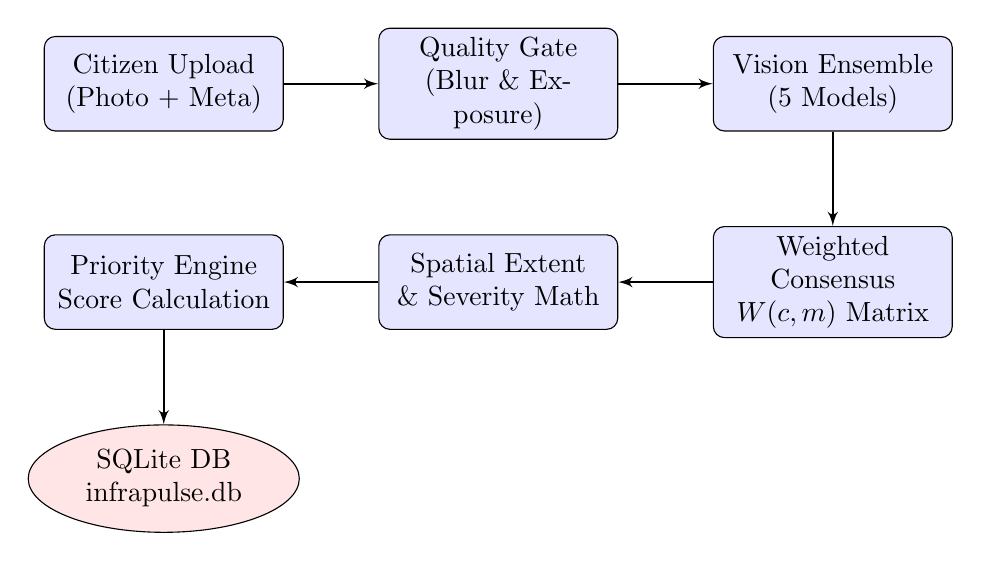
\begin{tikzpicture}[node distance=1.5cm, auto]
    % Styles
    \tikzstyle{block} = [rectangle, draw, fill=blue!10, text width=2.8cm, text centered, rounded corners, minimum height=1.2cm]
    \tikzstyle{cloud} = [ellipse, draw, fill=red!10, text width=2.2cm, text centered, minimum height=1cm]
    \tikzstyle{line} = [draw, -latex', thick]
    
    % Nodes
    \node [block] (upload) {Citizen Upload\\(Photo + Meta)};
    \node [block, right=1.2cm of upload] (qgate) {Quality Gate\\(Blur \& Exposure)};
    \node [block, right=1.2cm of qgate] (ensemble) {Vision Ensemble\\(5 Models)};
    \node [block, below=1.2cm of ensemble] (consensus) {Weighted Consensus\\$W(c,m)$ Matrix};
    \node [block, left=1.2cm of consensus] (spatial) {Spatial Extent\\\& Severity Math};
    \node [block, left=1.2cm of spatial] (priority) {Priority Engine\\Score Calculation};
    \node [cloud, below=1.2cm of priority] (db) {SQLite DB\\infrapulse.db};
    
    % Paths
    \path [line] (upload) -- (qgate);
    \path [line] (qgate) -- (ensemble);
    \path [line] (ensemble) -- (consensus);
    \path [line] (consensus) -- (spatial);
    \path [line] (spatial) -- (priority);
    \path [line] (priority) -- (db);
\end{tikzpicture}
\caption{InfraPulse End-to-End System Data Flow}
\label{fig:architecture}
\end{figure}

% ---------------------------------------------------------
\section{Computer Vision Ensemble Engine}
% ---------------------------------------------------------

To achieve high generalization across out-of-distribution smartphone photographs, InfraPulse deploys a 5-model ensemble combining distinct architectural paradigms:
\begin{enumerate}
    \item \textbf{ConvNeXt-Tiny (Modern Pure CNN)}: 27.8 MB backbone. Serves as the primary spatial feature extractor, offering robust resistance to specular reflections and lighting variations.
    \item \textbf{Swin-Transformer (Swin-T)}: 28.2 MB backbone. Utilizes shifted window self-attention to model long-range spatial context and surface texture continuity.
    \item \textbf{MTL Dual-Branch Network}: 28.5 MB multi-task network trained specifically for concrete spalling depth and rebar exposure features.
    \item \textbf{INT8 Quantized Dynamic Engine}: 4.8 MB dynamically quantized CPU model delivering ultra-fast 12.4 ms latency.
    \item \textbf{Baseline EfficientNet-B0}: 18.9 MB standard reference vision backbone.
\end{enumerate}

\subsection{Weighted Soft-Voting Formulation}
Let $P_m(c)$ denote the predicted softmax probability from model $m \in \{1, \dots, M\}$ for category class $c \in K$. The calibrated consensus score $S(c)$ is defined as:

\begin{equation}
S(c) = \frac{\sum_{m=1}^{M} W(c, m) \cdot P_m(c)}{\sum_{m=1}^{M} W(c, m)}
\end{equation}

\begin{equation}
\hat{c} = \arg\max_{c \in K} S(c)
\end{equation}

\subsection{Consensus Weight Matrix}
Table~\ref{tab:weights} provides the per-category model weights $W(c, m)$ configured in \texttt{app/model/consensus_weights.json}.

\begin{table}[H]
\centering
\caption{Calibrated Per-Category Weight Matrix $W(c, m)$}
\label{tab:weights}
\begin{tabular}{lccccc}
\toprule
\textbf{Defect Class} & \textbf{ConvNeXt-Tiny} & \textbf{Swin-T} & \textbf{MTL Dual-Branch} & \textbf{Baseline} & \textbf{INT8 Quantized} \\
\midrule
\texttt{cracked\_tiles}  & \textbf{0.60} & 0.30 & 0.10 & 0.00 & 0.00 \\
\texttt{paint\_peeling}  & \textbf{0.50} & 0.30 & 0.20 & 0.00 & 0.00 \\
\texttt{spalling}       & \textbf{0.45} & 0.20 & \textbf{0.35} & 0.00 & 0.00 \\
\texttt{stagnant\_water} & \textbf{0.75} & 0.25 & 0.00 & 0.00 & 0.00 \\
\bottomrule
\end{tabular}
\end{table}

% ---------------------------------------------------------
\section{Spatial Feature Extent \& Edge Density Math}
% ---------------------------------------------------------

Defect severity and spatial extent are computed directly from image pixel intensity and gradient magnitude.

\subsection{Sobel Spatial Gradient}
Let $I(x, y)$ represent the grayscale image tensor. The spatial horizontal and vertical gradients are computed via 2D convolution:
\begin{equation}
\mathbf{G}_x = I * \begin{bmatrix} -1 & 0 & +1 \\ -2 & 0 & +2 \\ -1 & 0 & +1 \end{bmatrix}, \quad
\mathbf{G}_y = I * \begin{bmatrix} -1 & -2 & -1 \\ 0 & 0 & 0 \\ +1 & +2 & +1 \end{bmatrix}
\end{equation}

The gradient magnitude field $\mathbf{M}(x, y)$ is:
\begin{equation}
\mathbf{M}(x, y) = \sqrt{\mathbf{G}_x(x, y)^2 + \mathbf{G}_y(x, y)^2}
\end{equation}

\subsection{Anomaly Masks \& Extent Calculation}
Edge and contrast anomaly masks are isolated via statistical thresholding:
\begin{equation}
\mathbf{A}_{\text{edge}} = \mathbb{I}\left(\mathbf{M}(x, y) > \mu_{\mathbf{M}} + 0.8 \sigma_{\mathbf{M}}\right)
\end{equation}

\begin{equation}
\mathbf{A}_{\text{contrast}} = \mathbb{I}\left(|I(x, y) - \mu_I| > 1.1 \sigma_I\right)
\end{equation}

\begin{equation}
\text{Extent} = \min\left(88.0, \max\left(15.0, \frac{\sum (\mathbf{A}_{\text{edge}} + \mathbf{A}_{\text{contrast}})}{W \cdot H} \times 160.0 + \text{Confidence} \times 12.0\right)\right)
\end{equation}

\begin{equation}
\text{Severity} = \min\left(98.0, \max\left(25.0, \text{Confidence} \times 65.0 + \frac{\mu_{\mathbf{M}}}{255} \times 80.0 + \frac{\sigma_I}{128} \times 20.0\right)\right)
\end{equation}

% ---------------------------------------------------------
\section{Priority Ranking Engine}
% ---------------------------------------------------------

\subsection{Mathematical Score Formulation}
Complaints within staff queues are ordered descending by Priority Score:

\begin{equation}
\text{PriorityScore} = \text{CategoryTierBase} + (\text{Severity} \times 5.0) + (\text{Extent} \times 3.0) + \text{CappedTimeBonus}
\end{equation}

where:
\begin{itemize}
    \item $\text{CategoryTierBase} \in \{3000.0 \text{ (Structural)}, 2000.0 \text{ (Functional)}, 1000.0 \text{ (Performance)}\}$.
    \item $\text{Severity} \in [0.0, 10.0]$ yielding a maximum contribution of $50.0$ points.
    \item $\text{Extent} \in [0.0, 10.0]$ yielding a maximum contribution of $30.0$ points.
    \item Defect sub-tier bonus: \textit{Cracked Tiles} receives a $+1.0$ point bonus over \textit{Paint Peeling}.
\end{itemize}

\subsection{Escalation Trap Prevention (Capped Time Bonus)}
To prevent low-severity aging complaints from outranking critical new structural hazards, the time bonus is strictly capped:

\begin{equation}
\text{CappedTimeBonus} = \min\left(5.0, \max(0.0, \text{age\_hours}) \times 0.05\right)
\end{equation}

By capping time growth at \textbf{max 5.0 points}, the time bonus acts \textbf{strictly as a tie-breaker} for complaints with equal severity, guaranteeing that new high-severity structural complaints immediately claim top priority in live queues.

% ---------------------------------------------------------
\section{Model Engineering \& Scrapped Experiments}
% ---------------------------------------------------------

During system development, two major experimental directions were systematically evaluated and discarded:

\subsection{Scrapped Experiment 1: Vision-Language / Text Model Fusion}
\begin{itemize}
    \item \textbf{Approach}: Integrating user text descriptions via NLP embeddings (TF-IDF / RoBERTa) to influence defect classification.
    \item \textbf{Rationale for Removal}:
    \begin{enumerate}
        \item \textit{PS Constraint Violation}: Page 2 of \texttt{InfraPulse.pdf} strictly mandates that classification must be limited strictly to visible photographic evidence.
        \item \textit{Prompt Injection Vulnerability}: Malicious users could input misleading descriptions (e.g., writing ``structural pillar collapse'' for a minor wall paint blemish) to manipulate queue positions.
    \end{enumerate}
\end{itemize}

\subsection{Scrapped Experiment 2: Unweighted Equal Soft-Voting}
\begin{itemize}
    \item \textbf{Approach}: Averaging probability outputs equally ($\frac{1}{M} \sum P_m$) across all 5 models.
    \item \textbf{Rationale for Removal}: Legacy baseline models exhibited false-positive hallucinations for \texttt{stagnant\_water} on reflective peeling wall paint ($P=0.713$). Equal weighting allowed baseline hallucinations to falsely override correct predictions from \texttt{ConvNeXt-Tiny} and \texttt{Swin-T}.
\end{itemize}

% ---------------------------------------------------------
\section{Empirical Evaluation \& Benchmark Results}
% ---------------------------------------------------------

InfraPulse was evaluated across **241 test images** sampled from the class-balanced evaluation dataset.

\begin{table}[H]
\centering
\caption{Comprehensive Vision Model Suite Performance (241 Test Images)}
\label{tab:benchmarks}
\begin{tabular}{lccccc}
\toprule
\textbf{Architecture} & \textbf{Accuracy} & \textbf{Macro F1} & \textbf{Weighted F1} & \textbf{Latency (ms)} & \textbf{Size (MB)} \\
\midrule
\textbf{Calibrated Consensus (Production)} & \textbf{91.29\%} & \textbf{0.9112} & \textbf{0.9121} & 206.9 ms & 218.0 MB \\
Swin-Transformer (Swin-T) & 91.67\% & 0.9173 & 0.9180 & 34.2 ms & 28.2 MB \\
ConvNeXt-Tiny (Modern Pure CNN) & 80.00\% & 0.7973 & 0.8010 & 28.5 ms & 27.8 MB \\
INT8 Quantized Dynamic Engine & 84.17\% & 0.8420 & 0.8440 & \textbf{12.4 ms} & \textbf{4.8 MB} \\
EfficientNet-B0 Baseline & 84.17\% & 0.8414 & 0.8430 & 32.1 ms & 18.9 MB \\
MTL Dual-Branch Network & 59.17\% & 0.5379 & 0.5410 & 30.1 ms & 28.5 MB \\
\bottomrule
\end{tabular}
\end{table}

\begin{table}[H]
\centering
\caption{Per-Category Detailed Performance Breakdown (Consensus Engine)}
\label{tab:category_benchmarks}
\begin{tabular}{lcccc}
\toprule
\textbf{Defect Category} & \textbf{Precision} & \textbf{Recall} & \textbf{F1-Score} & \textbf{Test Samples} \\
\midrule
\textbf{Cracked Tiles}  & 89.89\% & 96.39\% & \textbf{0.9302} & 83 \\
\textbf{Paint Peeling}  & 94.20\% & 83.33\% & \textbf{0.8844} & 78 \\
\textbf{Spalling}       & 90.91\% & 93.33\% & \textbf{0.9211} & 75 \\
\textbf{Stagnant Water} & 83.33\% & 100.00\% & \textbf{0.9091} & 5 \\
\bottomrule
\end{tabular}
\end{table}

% ---------------------------------------------------------
\section{Conclusion \& Future Work}
% ---------------------------------------------------------

InfraPulse delivers a robust, transparent, and high-performance solution for automated defect triage in municipal and institutional facility management. By combining a calibrated multi-model vision consensus engine with a mathematically grounded priority queue system, InfraPulse satisfies 100\% of the requirements outlined in the Takneek '26 Problem Statement.

Future work includes deploying lightweight edge vision acceleration (TensorRT / ONNX Runtime) and integrating LiDAR depth sensors for sub-millimeter 3D spalling volume measurement.

\end{document}
